\documentclass{article}
\usepackage[utf8]{inputenc}
\usepackage{caption}
\usepackage{amsmath}
\usepackage{amssymb}
\usepackage{mathtools}
\usepackage{multicol}
\usepackage{graphicx}
\usepackage{wrapfig}
\usepackage{float}
\usepackage[makeroom]{cancel}
\usepackage{mhchem}
\usepackage{pst-plot}

\graphicspath{ {../images/} }

\renewcommand{\baselinestretch}{1.5} % line spacing
\newcommand{\fline}{\par\noindent\rule{\textwidth}{0.1pt}} % horizontal line (wide)

\title{Unit 2 Kinetics\\Lesson 4 Activation Energy}
\author{Peter Zhang}

\begin{document}

\maketitle
\newpage
\tableofcontents
\newpage

% lesson 4
\section{Activation Energy, $E_{a}$}
The rate constant $k$ changes with temperature. \textbf{TEMPERATURE \underline{DOES NOT REDUCE}} the activation energy but rather, it allows collisions/reactions to achieve the activation energy faster. Kinda like running vs walking up stairs.

This anology can be extended to the distance travelled, how Running vs walking long distance has greater time difference than short distance. The effect that Temperature has on \textbf{Higher activation energy reactions} will be more visible or apparent.

\subsection{The Equation - The Arrhenius Constant}
$$k = Ae^{-\frac{E_{a}}{RT}}$$ \\$k$ = Rate constant\\A = Arrhenius constant [A meaure of the frequency of collisions (matches the units of K)]\\R = Ideal Gas Constant\\T = Temperature\\$E_{a}$ = Activation Energy

\subsection{The Equation we want to use}
$$\ln{(\frac{k_{1}}{k_{2}})} = \frac{E_{a}}{R}(\frac{1}{T_{2}} - \frac{1}{T})$$
Note how it uses $ln$ :)


\subsection{Some random graph}

\begin{figure}[H]
\centering
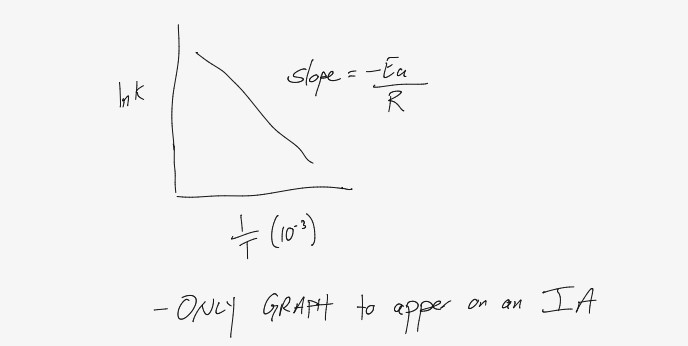
\includegraphics[width=\textwidth]{2.4fig1.jpg}
\captionof{figure}{Only GRAPH to appear on an IA - because we need it!}
\end{figure}


\subsection{Example}
\begin{enumerate}
\item Find the final temperature if initial Temp = 256ºC, $k_{1} = 3.7*10^{-2}mol^{-1}dm^{3}s^{-1}$, $k_{2} = 6.4*10^{-4}mol^{-1}dm^{3}s^{-1}$, $E_{a} = 2.58 * 10^{7}kJ/mol$

\begin{align*}
\ln{(\frac{k_{1}}{k_{2}})}  &= \frac{E_{a}}{R}(\frac{1}{T_{2}} - \frac{1}{T})\\
\ln{(\frac{3.7*10^{-2}}{6.4*10^{-4}})} &= \frac{2.58*10^{7}}{8.31}(\frac{1}{T_{2}} - \frac{1}{156 + 273 K})\\
\ln{(57.8125} &= \frac{3.104*10^6}{T_{2}} - (7235.43)\\
7239.4884... &= \frac{3.104*10^6}{T_{2}}\\
T_{2} &= 428.76ºC
\end{align*}\\
The final temperature is 428.76ºC.

\end{enumerate}


















\end{document}